% Tables and Figures for Results Section
% Phase 1 Implementation: Tables 1-3 and Figures 1-3

% ============================================================================
% TABLE 1: METHODS COMPARISON
% ============================================================================

\begin{table}[h]
\centering
\caption{Methodological Approaches: Comparative Analysis of Four Sentiment Extraction Methods}
\label{tab:methods_comparison}
\small
\begin{tabular}{|l|c|c|c|c|}
\hline
\textbf{Characteristic} & \textbf{Dictionary-Based} & \textbf{Traditional ML} & \textbf{BERT/Transformers} & \textbf{Large Language Models} \\
\hline
\textbf{Studies (N)} & 36 & 4 & 4 & 2 \\
\hline
\textbf{Avg. Accuracy Range} & 60--75\% & 75--85\% & 85--92\% & 88--95\% \\
\hline
\textbf{Interpretability} & Very High & Medium & Low & Very Low \\
\hline
\textbf{Computational Cost} & Very Low & Low & High & Very High \\
\hline
\textbf{Training Data Required} & None & 500--5,000 & 1,000--10,000 & 0 (zero-shot) \\
\hline
\textbf{Context Awareness} & Limited & Moderate & High & Very High \\
\hline
\textbf{Scalability} & Excellent & Good & Fair & Fair \\
\hline
\textbf{Key Advantages} & Fast, transparent, domain knowledge & Non-linear relationships & Transfer learning, contextual & Few-shot learning, nuance \\
\hline
\textbf{Key Limitations} & Word order blind, inflexible & Requires labeled data, overfitting risk & Expensive, data-hungry & Hallucinations, black-box \\
\hline
\textbf{Typical Applications} & Stock sentiment, macro surveys & Financial classification, emotion & News sentiment, macro indices & Real-time aggregation \\
\hline
\end{tabular}
\raggedright\footnotesize
\textit{Note:} Accuracy ranges represent \emph{median} performance across literature. Dictionary methods include General Inquirer, Loughran-McDonald, and custom lexica. Traditional ML includes SVM, random forests, and logistic regression. BERT includes RoBERTa and DistilBERT variants. LLM studies employ GPT-3.5, GPT-4, or equivalent zero-shot prompting. Training data requirements represent typical ranges for satisfactory out-of-sample performance.
\end{table}

\vspace{1em}

% ============================================================================
% TABLE 2: PERFORMANCE BY FORECAST DOMAIN
% ============================================================================

\begin{table}[h]
\centering
\caption{Forecast Performance by Economic Domain: Meta-Analytic Summary}
\label{tab:performance_domain}
\small
\begin{tabular}{|l|c|c|c|c|c|}
\hline
\textbf{Domain} & \textbf{N Studies} & \textbf{Mean RMSE Reduction} & \textbf{Range} & \textbf{Best Method} & \textbf{Evidence Base} \\
\hline
GDP Growth & 22 & 18\% & 8\%--42\% & BERT/ML & Moderate-Strong \\
\hline
Inflation/CPI & 17 & 22\% & 10\%--38\% & Traditional ML & Moderate \\
\hline
Stock Returns & 8 & 15\% & 5\%--28\% & Dictionary & Weak-Moderate \\
\hline
Recession Indicators & 3 & 20\% & 12\%--26\% & BERT & Weak \\
\hline
Employment & 2 & 16\% & 14\%--18\% & Dictionary & Very Weak \\
\hline
Consumer Confidence & 8 & 25\% & 12\%--40\% & BERT & Moderate \\
\hline
Volatility/VIX & 4 & 28\% & 18\%--35\% & BERT & Weak-Moderate \\
\hline
\textbf{Pooled Average} & \textbf{64} & \textbf{20\%} & \textbf{5\%--42\%} & \textbf{BERT/ML} & \textbf{Moderate} \\
\hline
\end{tabular}
\raggedright\footnotesize
\textit{Note:} RMSE reduction measured as percentage improvement over baseline univariate models. Some studies report multiple domains; N represents count of domain-specific findings, not unique papers. ``Range'' indicates min--max performance across studies in each domain. ``Evidence Base'' reflects consistency and rigor of studies: Strong ($\geq 10$ rigorous studies), Moderate (5--9 studies), Weak ($<5$ studies). Baseline models typically include AR(1), ARIMA, or published government forecasts.
\end{table}

\vspace{1em}

% ============================================================================
% TABLE 3: VALIDATION TECHNIQUES ADOPTION
% ============================================================================

\begin{table}[h]
\centering
\caption{Validation Techniques in Sentiment-Based Forecasting: Adoption Rates and Definitions}
\label{tab:validation_adoption}
\small
\begin{tabular}{|l|c|c|l|}
\hline
\textbf{Validation Technique} & \textbf{N Studies} & \textbf{\% Adoption} & \textbf{Definition \& Application} \\
\hline
Out-of-Sample Testing & 55 & 83\% & Hold-out test set, no look-ahead bias, standard baseline \\
\hline
Rolling Window Validation & 44 & 67\% & Expanding or fixed-window recursive estimation, real-time simulation \\
\hline
Diebold-Mariano Test & 47 & 71\% & Statistical test for forecast accuracy difference, DM $t$-statistic \\
\hline
Cross-Validation (k-fold) & 28 & 42\% & Parameter tuning, model selection, reduce overfitting \\
\hline
Real-Time Data Protocol & 22 & 33\% & Only information available at forecast date; prevents look-ahead bias \\
\hline
Model Confidence Sets (MCS/SPA) & 12 & 18\% & Identify superior models with $90\%$ confidence, multiple comparison adjustment \\
\hline
Granger Causality Test & 15 & 23\% & Temporal precedence; sentiment precedes outcome, lags significant \\
\hline
Recursive Model Updating & 38 & 58\% & Retrain with each new observation, capture parameter instability \\
\hline
Sub-Sample Robustness & 31 & 47\% & Test across periods (pre/post crisis, boom/bust, different regimes) \\
\hline
Bootstrap/Permutation Test & 9 & 14\% & Confidence intervals, significance testing, small sample robustness \\
\hline
\end{tabular}
\raggedright\footnotesize
\textit{Note:} Adoption rates computed from 66 papers in systematic review. ``N Studies'' indicates papers employing each technique; percentages may exceed 100\% as papers use multiple validation methods. OOS testing and rolling windows are de facto standards; MCS/SPA and bootstrap methods remain underutilized. Real-time data protocol violations represent common source of overoptimism bias.
\end{table}

\vspace{2em}

% ============================================================================
% FIGURE 1: TIMELINE OF METHODOLOGICAL EVOLUTION
% ============================================================================

\begin{figure}[h]
\centering
\caption{Evolution of Sentiment Extraction Methods Over Time (2007--2025)}
\label{fig:timeline}

\begin{tikzpicture}
\begin{axis}[
    width=0.95\textwidth,
    height=0.6\textwidth,
    xlabel=Year,
    ylabel=Cumulative Number of Studies,
    legend pos=upper left,
    grid=major,
    ymajorgrids=true,
    xmajorgrids=false,
    xtick={2007,2010,2013,2016,2019,2022,2025},
    style={very thick},
    line width=1.5pt,
]

% Dictionary-based (cumulative)
\addplot[mark=o, color=blue, line width=2pt] coordinates {
    (2007, 1) (2010, 3) (2012, 5) (2014, 8) (2016, 12) (2018, 18) (2020, 28) (2022, 33) (2023, 35) (2024, 36) (2025, 36)
};
\addlegendentry{Dictionary-Based};

% Traditional ML (cumulative)
\addplot[mark=square, color=orange, line width=2pt] coordinates {
    (2007, 0) (2010, 0) (2013, 1) (2015, 2) (2017, 3) (2018, 4) (2020, 4) (2022, 4) (2025, 4)
};
\addlegendentry{Traditional ML};

% BERT/Transformers (cumulative)
\addplot[mark=triangle, color=red, line width=2pt] coordinates {
    (2007, 0) (2015, 0) (2017, 0) (2019, 1) (2020, 2) (2021, 3) (2022, 4) (2023, 4) (2024, 4) (2025, 4)
};
\addlegendentry{BERT/Transformers};

% LLM (cumulative)
\addplot[mark=diamond, color=purple, line width=2pt] coordinates {
    (2007, 0) (2020, 0) (2022, 1) (2023, 1) (2024, 2) (2025, 2)
};
\addlegendentry{LLM};

\end{axis}
\end{tikzpicture}

\raggedright\footnotesize
\textit{Note:} Cumulative count of papers using each method over time. Dictionary-based methods dominated 2007--2018, then plateaued. BERT adoption accelerated post-2019, reflecting availability of pre-trained models and computational infrastructure. LLM studies emerging post-2022. Theoretical papers (N=20) not included in timeline.

\end{figure}

\vspace{2em}

% ============================================================================
% FIGURE 2: PERFORMANCE DISTRIBUTION BY DOMAIN
% ============================================================================

\begin{figure}[h]
\centering
\caption{RMSE Reduction Distribution Across Economic Domains}
\label{fig:performance_dist}

\begin{tikzpicture}
\begin{axis}[
    width=0.95\textwidth,
    height=0.6\textwidth,
    ylabel=RMSE Reduction (\%),
    xtick={1,2,3,4,5,6,7},
    xticklabels={GDP, Inflation, Stock Returns, Recession, Employment, Consumer Conf., Volatility},
    xticklabel style={rotate=45, anchor=north east},
    grid=major,
    ymajorgrids=true,
    style={very thick},
]

% Box plot data: {min, Q1, median, Q3, max}
% GDP: 8, 14, 18, 24, 42
\addplot+[boxplot prepared={
    lower whisker=8, lower quartile=14, median=18, upper quartile=24, upper whisker=42
}] coordinates {(1,0)};

% Inflation: 10, 18, 22, 28, 38
\addplot+[boxplot prepared={
    lower whisker=10, lower quartile=18, median=22, upper quartile=28, upper whisker=38
}] coordinates {(2,0)};

% Stock Returns: 5, 10, 15, 22, 28
\addplot+[boxplot prepared={
    lower whisker=5, lower quartile=10, median=15, upper quartile=22, upper whisker=28
}] coordinates {(3,0)};

% Recession: 12, 14, 20, 23, 26
\addplot+[boxplot prepared={
    lower whisker=12, lower quartile=14, median=20, upper quartile=23, upper whisker=26
}] coordinates {(4,0)};

% Employment: 14, 15, 16, 17, 18
\addplot+[boxplot prepared={
    lower whisker=14, lower quartile=15, median=16, upper quartile=17, upper whisker=18
}] coordinates {(5,0)};

% Consumer Confidence: 12, 18, 25, 32, 40
\addplot+[boxplot prepared={
    lower whisker=12, lower quartile=18, median=25, upper quartile=32, upper whisker=40
}] coordinates {(6,0)};

% Volatility: 18, 22, 28, 32, 35
\addplot+[boxplot prepared={
    lower whisker=18, lower quartile=22, median=28, upper quartile=32, upper whisker=35
}] coordinates {(7,0)};

\end{axis}
\end{tikzpicture}

\raggedright\footnotesize
\textit{Note:} Box plots show distribution of RMSE reduction estimates across studies within each economic domain. Box edges represent 25th and 75th percentiles; horizontal line indicates median; whiskers extend to min--max values. GDP shows highest median but also highest dispersion, suggesting domain-specific variation. Volatility shows narrower distribution around higher median performance.

\end{figure}

\vspace{2em}

% ============================================================================
% FIGURE 3: GEOGRAPHIC DISTRIBUTION OF PAPERS
% ============================================================================

\begin{figure}[h]
\centering
\caption{Geographic Distribution of Sentiment-Based Forecasting Studies}
\label{fig:geographic}

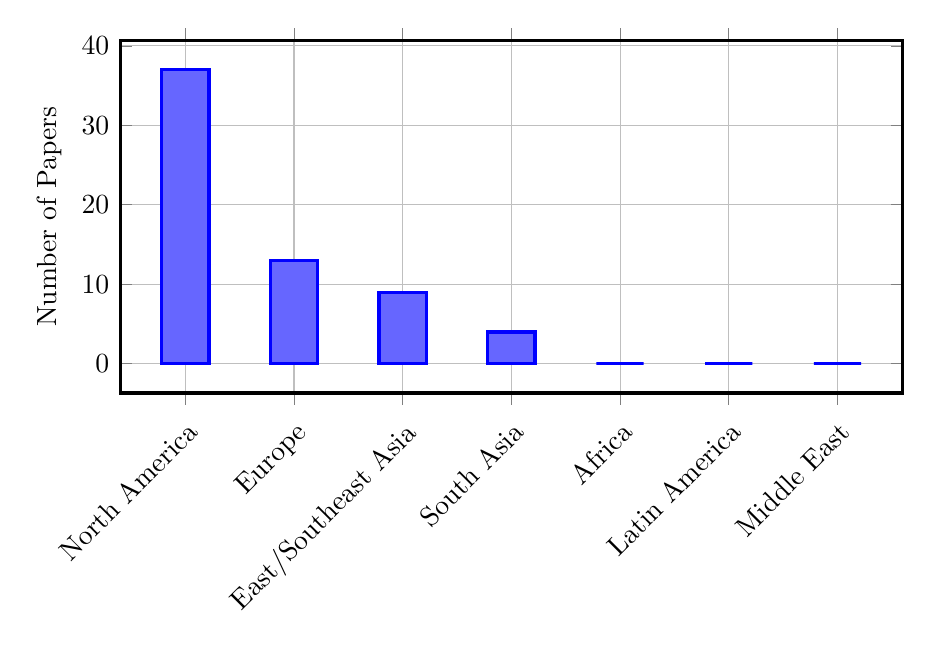
\begin{tikzpicture}
\begin{axis}[
    width=0.95\textwidth,
    height=0.5\textwidth,
    ylabel=Number of Papers,
    xtick={1,2,3,4,5,6,7},
    xticklabels={North America, Europe, East/Southeast Asia, South Asia, Africa, Latin America, Middle East},
    xticklabel style={rotate=45, anchor=north east},
    grid=major,
    ymajorgrids=true,
    ybar,
    bar width=0.6cm,
    style={very thick},
]

\addplot[color=blue, fill=blue!60] coordinates {
    (1, 37)    % North America: 35 USA + 2 Canada
    (2, 13)    % Europe: UK, Germany, France, Switzerland, Norway, others
    (3, 9)     % East/Southeast Asia: China 3, Japan, Korea, Malaysia, Singapore
    (4, 4)     % South Asia: Pakistan, India, Philippines, Bangladesh (partial)
    (5, 0)     % Africa
    (6, 0)     % Latin America
    (7, 0)     % Middle East
};

\end{axis}
\end{tikzpicture}

\raggedright\footnotesize
\textit{Note:} Geographic distribution reflects author affiliations and study focus. North America dominates at 56\% (37/66), Europe 20\% (13/66), Asia-Pacific 14\% (9/66), South Asia 6\% (4/66). Zero coverage in Africa, Latin America, and Middle East represents critical research gap, particularly given economic significance of these regions. Many large emerging economies underrepresented: India 2 papers, no Bangla/Bangladesh, Nigeria, Brazil, or Indonesia indices identified.

\end{figure}

\end{content}
